\begin{enumerate}
	\item To decide whether there exists $k$ edge-disjoint paths, we can define the capacity of each edge as 1. Thus the flow will only go through an edge at most 1 time. Then we push the maximum flow possible from s. It means a flow of $n=degree(s)$. So the maximum number of edge-disjoint paths is bounded by $n$. Then we see how many of the incoming edges of $t$ will be used and check if it's bigger or equal to $k$. It means we pass through at most $|E|$ edges. So this algorithm runs in polynomial time.
	\item To check if there are $k$ node-disjoint paths, we can use the same algorithm as before but every time we reach a node (which is not $t$) by a given edge, we need to set the capacity of its other incoming edges (obviously if the in-degree of the node is bigger than 1) to 0. So a node can be accessed only 1 time. Then we see how many of the incoming edges of $t$ will be used and check if it's bigger or equal to $k$. The algorithm runs in polynomial time since we visit at most $|V|$ nodes but we need also to change capacity of at most $|V|$ incoming edges.
	\item Let's define $E_1$ as the set of all edges from $s$ to $u$ and $E_2$ the set of edges from $u$ to $t$. Since it's a directed graph, $E_1$ and $E_2$ are disjoint if there is no cycle. It means one of the $k$ paths from $s$ to $u$ will not share any edge with one of the $k$ paths from $u$ to $t$. So from $s$ to $t$ we have at least $k$ paths ("at least" because there may exist one or many paths from $s$ to $t$ that don't pass by $u$). In case of a cycle like we can see on Figure \ref{fig:cycle}, from $u$ to $t$ we don't have more edge-disjoint paths with or without this cycle, so this cycle can be ignored.
	\begin{figure}[ht]
  \centering
  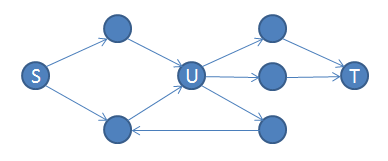
\includegraphics[width=0.5\textwidth]{cycle}
  \caption{Example of a cycle}
  \label{fig:cycle}
  \end{figure}
	\item The counter example in Figure \ref{fig:prob1} shows that a directed graph may have $k$ paths from $s$ to $u$ and k paths from $u$ to $t$ but there are less paths from $s$ to $t$.
	\begin{figure}[ht]
  \centering
  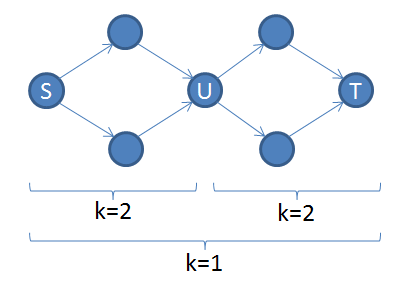
\includegraphics[width=0.5\textwidth]{prob1}
  \caption{A counter example}
  \label{fig:prob1}
  \end{figure}
\end{enumerate}